\section{Background Knowledge}

\subsection{Eye movements}
To understand how speed reading is possible, it's important to know some basics on how the eye moves.

When you read, visually analyse or look for something, your eyes are doing a series of movements called \textit{saccades}. Between these movements, your eyes shortly fixate on elements. These stops are called \textit{fixations}. Each fixations lasts only around 200-300 ms, so our eyes are quickly looking around a scene to find new details to fixate on. The movements of the eyes  are incredibly fast, reaching speeds of 500 degrees a second \cite{eyeMovement}.


But this all depends on what you're using your eyes for. There is generally three types of saccades: pursuit, vergence and vestibular. \textit{Pursuit} is when your eyes are trying to fixate on something moving. Generally, in these cases, the saccades are slower, as your eyes are following the target and not going back and forth between different targets \cite{eyeMovement}.
\textit{Vergence} is the inwards movement of your eyes to focus on something getting closer to you \cite{eyeMovement}.

\textit{Vestibular} movement is the eyes rotating to compensate for body and/or head movement. This is both caused by visual stimulation, but mostly by the vestibular organ in your ears. This is also also why your sight gets blurry when you're dizzy.

In the case of reading, it's also important to talk about the different kinds of small saccades the eyes are capable of. \textit{Nystagmus} are tiny and quick movements in the eyes, which causes a tremor in your vision \cite{eyeMovement}. You will notice it when staring intently at a fixed point. It's believed that this is a precaution in the eyes to make the nerve cells keep firing by continuously stimulating them. Furthermore, the eyes also experience small \textit{drifts}. These are believed to be the results of a less-than-perfect control of the oculomotor, resulting in the eyes slowly drifting to one side. To accommodate this, the eyes make tiny saccades, called \textit{microsaccades}, to realign themselves \cite{eyeMovement}. 

Another aspect to understand is \textit{saccade latency}. Every time a saccade is made, some calculations are needed to approximate where to move the eyes to fixate on a desired target. Even if excluding the uncertainty of where to move the eyes, it would still take 150-175 ms for the initial "request" of moving the eyes to the actual start of the movement. Cognitive processes further increases this latency, but also increases accuracy, meaning your fixation falls closer to the point of interest.

\textbf{(Gustav: maybe write something about cognitive processes from Perception book here)}

During the saccade, though, everything is a blur. Or it should be anyway. It seems certain parts associated with processing visual inputs are halted during saccades. This process is called \textit{saccadic suppression}. This is independent of the lexical processing, which means a reader is able to process read text in parallel with saccades \cite{eyeMovement}.

A fixation is not needed to read a word, though. Your attention can be shifted to objects or words in your peripheral vision. But it is not possible to make a saccade without shifting attention to the fixation.

\subsection{Optimal Recognition Position} \label{ORP}
The destination of each saccade when reading, or the fixation point, depends on the content of the sentence; sometimes, the eye also skip words by saccading past them. 80\% of the fixation points are on content words (nouns, verbs and adjectives) and the remaining 20\% are on articles, pronouns, and conjunctions \cite{eysenck_cognitive_2010}. The fixation point inside the words themselves, the \textit{optimal recognition position} (ORP), has an impact on how fast a reader can name the word they are looking at. Research has shown that the ORP is near the middle or slightly left of the middle \cite{oregan_optimal_1992, nazir_letter_1998, oregan_convenient_1984}. The added recognition time as the fixation point deviates from the ORP is a U-shaped curve, with around 20 ms added for each letter of deviation.

Not surprisingly removing the spacing between words decreases the reading speed with around 30\%. Fixation does not fall on the ORP but tends to the beginning of words. Interestingly enough adding spaces in long words, like long Danish or German compound words, actually increased reading speed, even though it was grammatically incorrect. Likewise with putting in spaces in Thai, where there are no spaces.

\textbf{(Gustav: maybe add an image of this curve?)}

\subsection{Attention}
MATHIAS

\subsection{Reading Processes}
\citeA{carver_reading_1992} presents five reading processes, also referred to as \textit{gears} (see Figure \ref{fig:trace_cross}). Each gear is defined by its \textit{goal}, \textit{culminating component}, and its \textit{speed}, measured by \textit{WPM} (words per minute). WPM also varies based on reading level, so to block out this bias, \citeauthor{carver_reading_1992} bases his experiments exclusively on college students. The following section is based on his study.

\begin{figure}[htbp]
\centering
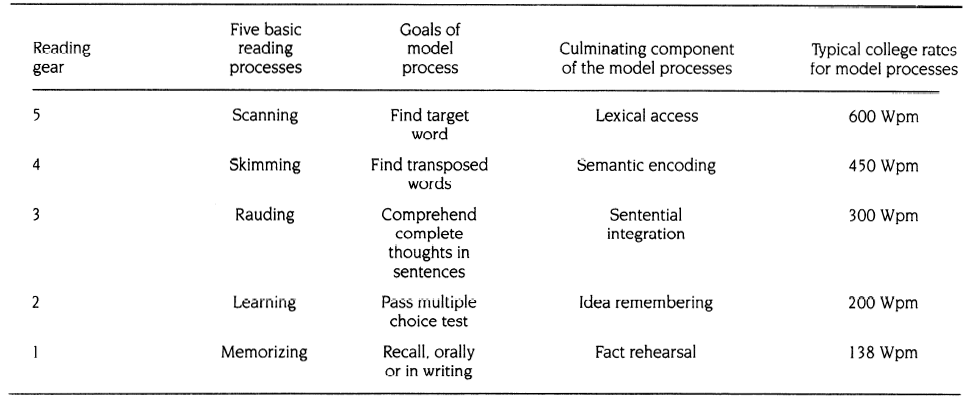
\includegraphics[width=0.5\textwidth]{Pics/gears_list}
\caption{Each gear has its own goal, culminating component, and WPM.}
\label{fig:gears_list}
\end{figure}

The goal relies on the reader's intent when reading the text. For instance, the reader could read the text just to find a single word (scanning). The culminating component of a gear, is then the cognitive process that it requires. \textit{Lexical access} is the component used for finding a single word in memory. If the reader's goal changed to finding a certain sentence in the text, such as in skimming, transposed words must be found and the activity would require an additional component; \textit{semantic encoding}. Other than just finding the words, the reader must now determine the meaning of the sentence. In order for the reader to understand the complete thought of a sentence, the \textit{sentential integration} component must be added. These three components together are the requirement for the most basic and most used reading process - \textit{rauding}, also known as \textit{typical reading}. The word comes from a combination of 'auding' and 'reading', as they both share the same underlying comprehension processes. If the goal of reading the text is to learn, e.g., in order to answer a test, the \textit{idea remembering} component is added. In this gear, some words require re-reading and longer time to process. The final gear is focused around remembering the text and uses the \textit{fact rehearsal} component. This gear requires rehearsing the material and memorizing it. 
\citeA{carver_reading_1992} goes on to mention that the best readers shift up and down in gear while reading, based on the difficulty of the material - a term called \textit{process flexibility}. 

By having college students read a text followed by answering two multiple choice tests, as well as judging their own performance, \citeauthor{carver_reading_1992} tested efficiency at different reading rates. It was found that the students were most efficient at rates around 300 WPM - the rauding reading rate. This rate has therefore been referred to as the most optimal reading rate.
%Efficiency was calculated from the product of accuracy and reading rate, and the accuracy was determined through multiple-choice tests as well as self-judgement.

\citeauthor{carver_reading_1992} also mentions the term \textit{cognitive speed}, which acts as a limit of the reading speed. If the reader passes this limit, he will not be able to operate the culminating components successfully, resulting in a poor comprehension. The main concern however for most students is to make the reading speed reach the limit of the cognitive speed.

\textbf{(Gustav: maybe remove this quote?)}

\citeauthor{carver_reading_1992} describes how the \textit{rauding theory} relates to the \textit{schema theory}. The schema theory uses gears 1 and 2, but mainly focuses on how readers learn or memorize text. \citeA{widmayer_schema_2005} presents schema as a set of rules that help processing new information by interpreting and predicting situations occurring in the environment. Specifically for reading, \citeauthor{widmayer_schema_2005} claims that:

 \emph{''...Correspondingly, teachers of reading have found that activating a learner's schema enables them to better process information that they are reading. Therefore, many advocate teaching learners metacognitive strategies designed to activate one's schema before reading, such as reading heading and the title, looking a visuals in the text, and making predictions based on the title and pictures.''}

This might indicate that when using schema, readers use skimming or scanning before reading a text, but shift to the memorization and learning gears as soon as they start reading. It also indicated that a complete overview of the text can be relevant in some cases.

%(INSERT REF: Reading for One Second, One Minute, or One Year) compares four different theoretical perspectives in reading, each focusing on a certain style and speed of reading: Rauding, Verbal Efficiency, Schema, and Whole Language.

\subsection{Sub-vocalization}
When children learn to read, they typically do this by associating printed symbols with previously-acquired listening and speaking skills \cite{bruinsma_should_1980}. Even though this "silent reading" soon becomes inaudible, the movements of lips, tongue and larynx sometimes continue for many years. These small movements are known as \textit{sub-vocalization} \cite{bruinsma_should_1980}. It has been found that poor readers demonstrate a greater degree of sub-vocalization than proficient readers. It has been believed that lip movements and sub-vocalization should be suppressed, so as the reading rate will increase \cite{bruinsma_should_1980}. However, according to \citeA{j_covert_1970}, oral behaviour during silent performance of language tasks does indeed serve a language function. \citeauthor{j_covert_1970} concludes that increased covert oral behaviour is beneficial during silent reading: \emph{"The implications for the teacher, thus, is that she should not tamper with the child's subvocalization? It is likely that the child NEEDS to subvocalize while reading, in any event, the subvocalization naturally becomes reduced in time."} \cite{bruinsma_should_1980}. Even if there are ways to reduce sub-vocalization, it might not be desirable for readers that have difficulty comprehending even low-level material. Instead, they should be encouraged to sub-vocalize to ensure the maximum comprehension \cite{bruinsma_should_1980}.

%http://www.jstor.org/stable/20195232
%[Conclusions The evidence cited here should caution teachers to be very careful in their efforts to reduce subvocalization during silent reading. This should be done directly only with students who are otherwise compe tent readers and who are reading relatively easy material ...]
